\documentclass[12pt]{article}
\usepackage{a4wide}
\usepackage{NotationStyle}
\usepackage[english]{babel}
\usepackage{amsmath,amssymb,mathrsfs,mathtext}
\usepackage{graphics,graphicx,epsfig}
\usepackage{epstopdf}
\usepackage{fancybox,fancyhdr}
\usepackage{enumerate}
\usepackage{array}
\usepackage[normalem]{ulem}
\renewcommand{\baselinestretch}{1.13}
\begin{document}

\section{Time searies resampling}
For the time series of sample rate that is changing, unstable, non-rational to the common rate as well as for the time series with missing values the following procedure should be applied.

Let the time~$t$ be in continous set~$\mathbb{R}_+^1$ and the time series~$s$ be piece-wise constant. There are three possibilities to create such time series from a discrete-values one: 1) the constant goes after the sample~$s(t)$, 2) before the sample, 3) in the neighborhood of the sample. See red, green and blue lines in the Figure~\ref{fig_resamle1}.

\begin{figure}[!hp]
\centering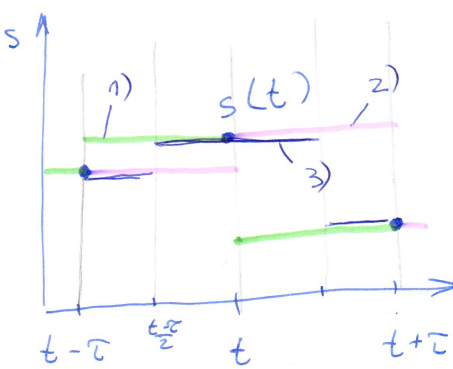
\includegraphics[width=0.5\textwidth]{resample1.png}
\label{fig_resamle1}
\caption{Piece-wise representation of a time series}
\end{figure}

This assumptions helps introducing a new sampling rate and eliminates the problem of missing values, since the previous (next, current in the terms of Fig.~\ref{fig_resamle1}) value holds continuously until the following comes. The constant model could be developed into more comples one: a piece-wise, quadratic or cubic spline with its nodes in the time-ticks or over the time-ticks according to the following criterions: 1) Nyquist�Shannon theorem, 2) Fisher-Neyman theorem. The following optimization problem returns the new sampling rate:
\[
\text{todo}
\]
This fixed rate is used to obtain a resampled time series with regular time-ticks.

\begin{figure}[!t]
\centering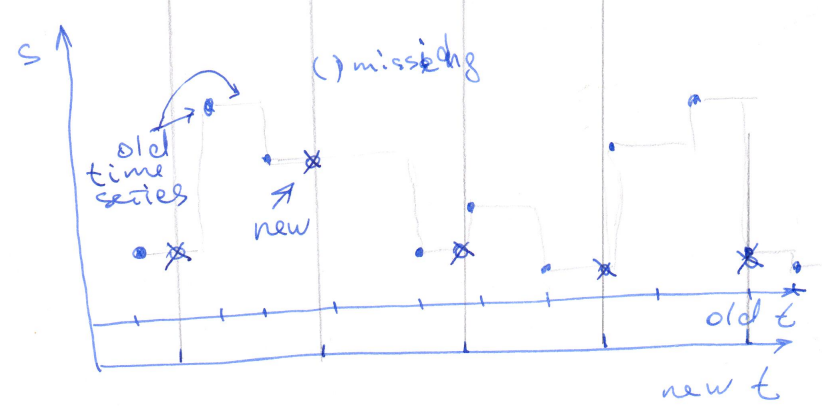
\includegraphics[width=0.9\textwidth]{resample2.png}
\label{fig_resamle2}
\caption{Resample time series of variating sample rate into the fixed one with the optimal period}
\end{figure}

\section{Nyquist�Shannon  resampling criterion}
todo

\section{ Fisher-Neyman resampling criterion}
todo

%\section{Resampling}
%Let us denote time-series $\bs$ and consider following cases:
%\begin{itemize}
%    \item Time-series $\bs$ has possesses clearly marked period. In this case non-overlaping samples can be used, their boundaries can be allocated according to the time-series period.
%    \item If time-series $\bs$ possesses weakly evident period or several different periods, samples can overlay to gain more information. Their boundaries, again, can be allocated according to the period.
%    \item In case when time-series $\bs$ doesn't possess any noticeable period, is too noisy or there is no information about time-series source, samples boundaries can be allocated in accordance with uniform distribution on timescale of  time-series $\bs$.
%\end{itemize}
%
%In general, the resampling parameters depends on the time-series properties and should be chosen according to the data source.
%
%Let us assume we know sampling frequency $\frac{1}{\tau}$, pre-history length $\Delta t_r$ and forecast horizon $\Delta t_p$. Then approximation function $\mathfrak{f}$ can be defined as:
%\begin{equation*}
%	\mathfrak{f}(\bs, t_i) = \bs(\hat{t}),
%\end{equation*}
%where $\hat{t}$ is the nearest time point, where $\bs$ value is determined. In other words, we approximate the time-series $\bs$ with a piecewise constant function possessing the value $\bs(\hat{t})$ on half-intervarls $[\hat{t}-T; \hat{t}+T)$, where $2T$ is the period of the time-series $\bs$.
%
%With setting sample size $l$ it's end-point $t_i$ with such conversion we get the sample itself:
%\begin{equation*}
%    \{\mathfrak{f}(t^*_j)\}_{j=1}^{l}, \; t^*_j \in [t_i - (\Delta t_p + \Delta t_r, t_i], \; j = \{1, \ldots, l \}.
%\end{equation*}
%
%After samples generation we get new object $\bx'$ and answer $\by'$ vectors. The object vectors contain first $\Delta t_r$ elements of samples, and the rest $\Delta t_p$ elements form the answer vectors.
%
%After or before resampling operation, additional features can be generated using various transformations with time-series components.




\end{document} 